% Capa
\imprimircapa

% Folha de rosto
% (o * indica que haverá a ficha bibliográfica)
\imprimirfolhaderosto

% Inserir a ficha bibliografica
% http://ficha.bu.ufsc.br/
%\begin{fichacatalografica}
%	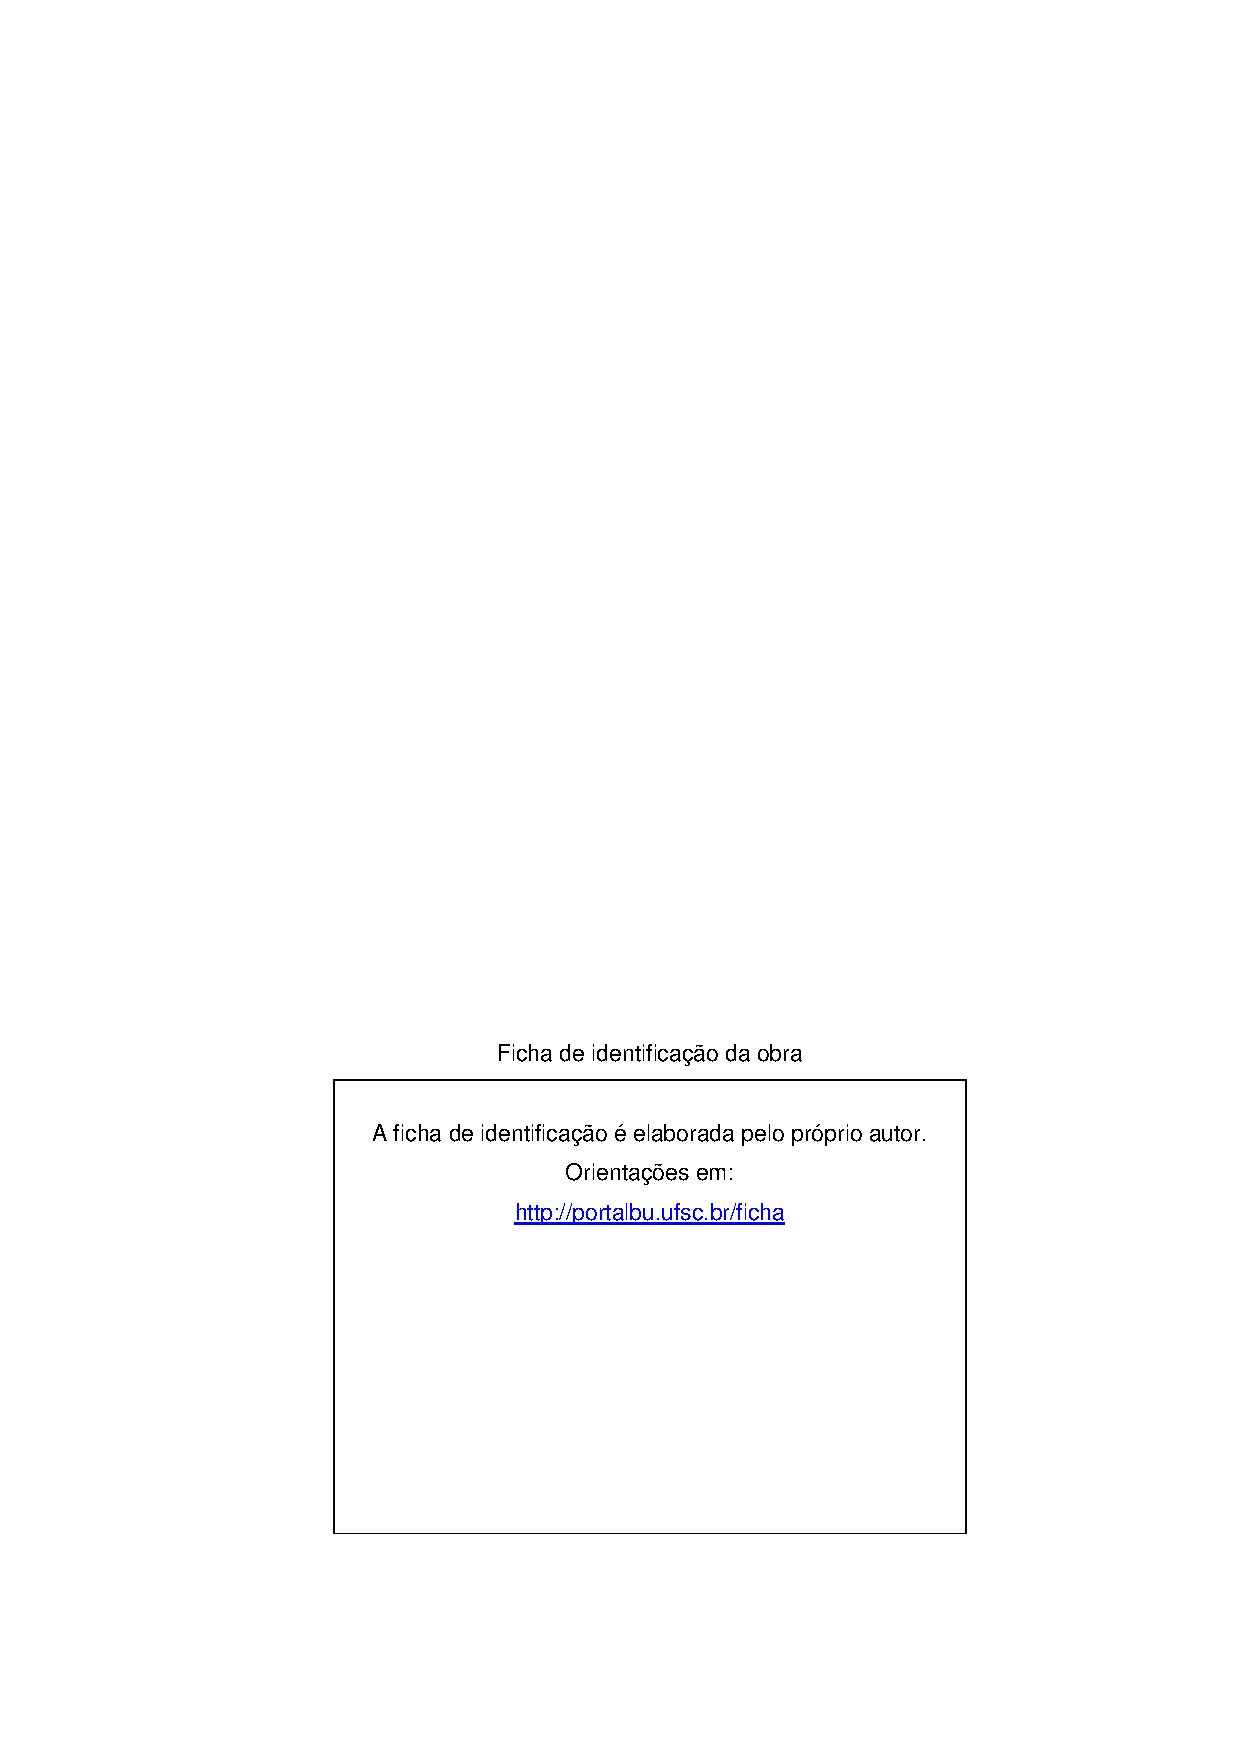
\includepdf{beforetext/Ficha_Catalografica.pdf}
%\end{fichacatalografica}

% Folha de aprovação
\begin{folhadeaprovacao}
	\small
	\begin{snugshade}
		\begin{center}
			{\textbf{FOLHA DE APROVAÇÃO DE PROPOSTA DE TCC}}
		\end{center}
	\end{snugshade}
	\vspace{-18pt}

	\footnotesize
	\begin{quadro}[htb]
		\centering
		\label{qua:folha_aprov}
		\begin{tabular}{|l|p{10.5cm}|}
			\hline
			\textbf{Acadêmico}            & \imprimirautor      \\ \hline
			\textbf{Título do trabalho}   & \imprimirtitulo     \\ \hline
			\textbf{Curso}                & \imprimirprograma   \\ \hline
			\textbf{Área de Concentração} & Visão computacional \\ \hline
		\end{tabular}
	\end{quadro}

	\vspace{-14pt}

	\noindent \textbf{Instruções para preenchimento pelo ORIENTADOR DO TRABALHO}:
	\begin{itemize}[leftmargin=*,noitemsep,topsep=0pt]
		\item[-] Para cada critério avaliado, assinale um X na coluna SIM apenas se considerado aprovado. Caso contrário, indique as alterações necessárias na coluna Observação.
	\end{itemize}

	\vspace{-4pt}

	\definecolor{Silver}{rgb}{0.752,0.752,0.752}
	\begin{table}[htb]
		\footnotesize
		\centering
		\begin{tblr}{
			width = \linewidth,
			colspec = {Q[452]Q[56]Q[85]Q[56]Q[150]Q[137]},
			row{1} = {Silver,c},
			row{2} = {Silver,c},
			cell{1}{1} = {r=2}{},
			cell{1}{2} = {c=4}{0.347\linewidth},
			cell{1}{6} = {r=2}{},
			cell{3}{2} = {Silver},
			cell{3}{3} = {Silver},
			cell{3}{4} = {Silver},
			cell{3}{5} = {Silver},
			cell{4}{2} = {Silver},
			cell{4}{3} = {Silver},
			cell{4}{4} = {Silver},
			cell{4}{5} = {Silver},
			cell{5}{2} = {Silver},
			cell{5}{3} = {Silver},
			cell{5}{4} = {Silver},
			cell{5}{5} = {Silver},
			cell{6}{2} = {Silver},
			cell{6}{3} = {Silver},
			cell{6}{4} = {Silver},
			cell{6}{5} = {Silver},
			cell{7}{2} = {Silver},
			cell{7}{3} = {Silver},
			cell{7}{4} = {Silver},
			cell{7}{5} = {Silver},
			cell{8}{2} = {Silver},
			cell{8}{3} = {Silver},
			cell{8}{4} = {Silver},
			cell{8}{5} = {Silver},
			cell{9}{2} = {Silver},
			cell{9}{3} = {Silver},
			cell{9}{4} = {Silver},
			cell{9}{5} = {Silver},
			cell{10}{2} = {Silver},
			cell{10}{3} = {Silver},
			cell{10}{4} = {Silver},
			cell{10}{5} = {Silver},
			cell{11}{2} = {Silver},
			cell{11}{3} = {Silver},
			cell{11}{4} = {Silver},
			cell{11}{5} = {Silver},
			cell{12}{2} = {Silver},
			cell{12}{3} = {Silver},
			cell{12}{4} = {Silver},
			cell{12}{5} = {Silver},
			cell{13}{2} = {Silver},
			cell{13}{3} = {Silver},
			cell{13}{4} = {Silver},
			cell{13}{5} = {Silver},
			cell{14}{2} = {Silver},
			cell{14}{3} = {Silver},
			cell{14}{4} = {Silver},
			cell{14}{5} = {Silver},
			cell{15}{2} = {Silver},
			cell{15}{3} = {Silver},
			cell{15}{4} = {Silver},
			cell{15}{5} = {Silver},
			vlines,
			hline{1,3-16} = {-}{},
					hline{2} = {2-5}{},
				}
			\textbf{Critérios }                                                                                                                                                                                                                                                                                & \textbf{Aprovado } &                  &              &                        & \textbf{Observação } \\
			                                                                                                                                                                                                                                                                                                   & \textbf{Sim}       & \textbf{Parcial} & \textbf{Não} & \textbf{Não se aplica} &                      \\
			{1. O trabalho é adequado para um TCC no CCO/SIN (relevância / abrangência)?}                                                                                                                                                                                                                      &                    &                  &              &                        &                      \\
			2. O titulo do trabalho é adequado?                                                                                                                                                                                                                                                                &                    &                  &              &                        &                      \\
			{3. O tema de pesquisa está claramente descrito?}                                                                                                                                                                                                                                                  &                    &                  &              &                        &                      \\
			{4. O problema/hipóteses de pesquisa do trabalho está claramente identificado?}                                                                                                                                                                                                                    &                    &                  &              &                        &                      \\
			5. A relevância da pesquisa é justificada?                                                                                                                                                                                                                                                         &                    &                  &              &                        &                      \\
			{6. Os objetivos descrevem completa e claramente o que se pretende alcançar neste trabalho?}                                                                                                                                                                                                       &                    &                  &              &                        &                      \\
			{7. É definido o método a ser adotado no trabalho? O método condiz com os objetivos e é adequado para um TCC?}                                                                                                                                                                                     &                    &                  &              &                        &                      \\
			{8. Foi definido um cronograma coerente com o método definido (indicando todas as atividades) e com as datas das entregas (p.ex. Projeto I, II, Defesa)?}                                                                                                                                          &                    &                  &              &                        &                      \\
			{9. Foram identificados custos relativos à execução deste trabalho (se houver)? Haverá financiamento para estes custos?}                                                                                                                                                                           &                    &                  &              &                        &                      \\
			{10. Foram identificados todos os envolvidos neste trabalho?}                                                                                                                                                                                                                                      &                    &                  &              &                        &                      \\
			{11. As formas de comunicação foram definidas (ex: horários para orientação)?}                                                                                                                                                                                                                     &                    &                  &              &                        &                      \\
			{12. Riscos potenciais que podem causar desvios do plano foram identificados?}                                                                                                                                                                                                                     &                    &                  &              &                        &                      \\
			{13. Caso o TCC envolva a produção de um software ou outro tipo de produto e seja desenvolvido também como uma atividade realizada numa empresa ou laboratório, consta da proposta uma declaração (Anexo 3) de ciência e concordância com a entrega do código fonte e/ou documentação produzidos?} &                    &                  &              &                        &
		\end{tblr}
	\end{table}

	\vspace{-4pt}

	\tiny
	\noindent \begin{tabularx}{\textwidth}{| l | X | l | l |}
		\hline
		{\textbf{Avaliação}}             & \multicolumn{1}{l}{\textbf{$\Box$ \tiny Aprovado}} & \multicolumn{2}{c|}{\textbf{$\Box$ \tiny Não Aprovado}}   \\ \hline \hline
		{\textbf{Professor Responsável}} & {...}                                              & {00/00/2024}                                            & \\ \hline
		{\textbf{Orientador}}            & {Prof. Dr. rer.nat. Aldo von Wangenheim}           & {00/00/2024}                                            & \\ \hline
	\end{tabularx}
\end{folhadeaprovacao}

% Resumo em português
\setlength{\absparsep}{18pt}
\begin{resumo}
	\SingleSpacing

	Considerando o aumento significativo observado no consumo e compartilhamento de vídeos nos últimos anos, é notória a demanda por técnicas que permitam armazenamento, transmissão e reprodução desse tipo de dado de forma cada vez mais otimizada.
	Para essa finalidade, a abordagem mais consolidada é a codificação de vídeo híbrida, que tem sido parte essencial da área de codificação de vídeo nas últimas décadas.
	Contudo, estima-se que a complexidade de algoritmos tradicionais híbridos venha aumentando em 10X para um ganho de desempenho de 2X, a cada geração.
	Nesse contexto, surge a necessidade de buscar modelos alternativos de codificação, como o \ac{DIVC}.
	O \ac{DIVC} combina o modelo de codificação híbrido com \ac{VFI}, porém tem desempenho variável de acordo com o conteúdo do vídeo.
	Portanto, o objetivo deste trabalho é propor uma técnica para melhorar sua eficiência de codificação a partir da remoção de quadros de forma adaptativa. Para isso, os quadros serão analisados utilizando descritores que apresentem melhor correlação com a eficiência do modelo.

	\textbf{Palavras-chave:} Codificação de vídeo. VVC. Eficiência de codificação. Descritores de imagem. VFI. Redes Neurais.
\end{resumo}

% resumo em inglês
%\begin{resumo}[Abstract]
%	\SingleSpacing
%	\begin{otherlanguage*}{english}
%		Resumo traduzido para outros idiomas, neste caso, inglês. Segue o formato do resumo feito na língua vernácula. As palavras-chave traduzidas, versão em língua estrangeira, são colocadas abaixo do texto precedidas pela expressão “Keywords”, separadas por ponto.

%		\textbf{Keywords}: Keyword 1. Keyword 2. Keyword 3.
%	\end{otherlanguage*}
%\end{resumo}

{%hidelinks
\hypersetup{hidelinks}
% ---
% inserir lista de ilustrações
% ---
\pdfbookmark[0]{\listfigurename}{lof}
% \listoffigures*
\cleardoublepage
% ---

% ---
% inserir lista de quadros
% ---
%\pdfbookmark[0]{\listofquadrosname}{loq}
%\listofquadros*
%\cleardoublepage
% ---

% ---
% inserir lista de tabelas
% ---
%\pdfbookmark[0]{\listtablename}{lot}
%\listoftables*
%\cleardoublepage
% ---

% ---
% inserir lista de abreviaturas e siglas (devem ser declarados no preambulo)
% ---
\imprimirlistadesiglas
% ---

% ---
% inserir lista de símbolos (devem ser declarados no preambulo)
% ---
%\imprimirlistadesimbolos
% ---

% ---
% inserir o sumario
% ---
\pdfbookmark[0]{\contentsname}{toc}
\tableofcontents*
\cleardoublepage

}%hidelinks
